\documentclass{article}
\usepackage{tikz}
\usetikzlibrary{matrix,arrows,decorations.pathmorphing}

\title{Category Theory \\ Cheat Sheet}
\author{Arnaud Bailly - Christophe Thibaut}
\date{01/12/2011}

\begin{document}

\begin{figure}
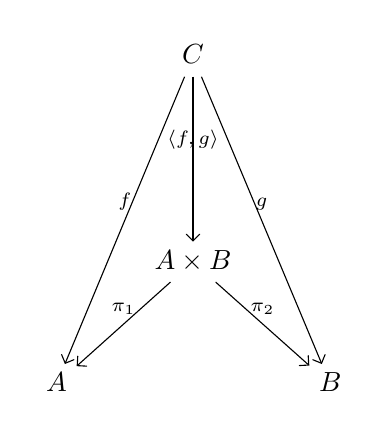
\begin{tikzpicture}[>=angle 90]
\matrix(a)[matrix of math nodes,
row sep=3em, column sep=2.5em,
text height=1.5ex, text depth=0.25ex]
{
&C& \\
\\
&A \times B&\\
A&&B\\};
\path[->,font=\scriptsize](a-1-2) edge node[above]{$f$} (a-4-1);
\path[->,font=\scriptsize](a-1-2) edge node[above]{$g$} (a-4-3);
\path[->,font=\scriptsize](a-1-2) edge node[above]{$\langle f, g\rangle$} (a-3-2);
\path[->,font=\scriptsize](a-3-2) edge node[above]{$\pi_1$} (a-4-1);
\path[->,font=\scriptsize](a-3-2) edge node[above]{$\pi_2$} (a-4-3);
\end{tikzpicture}
\caption{Product}
\end{figure}

\begin{figure}
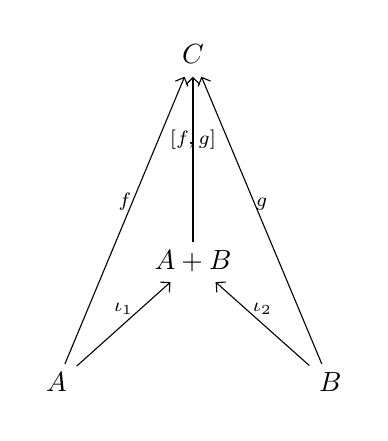
\begin{tikzpicture}[>=angle 90]
\matrix(a)[matrix of math nodes,
row sep=3em, column sep=2.5em,
text height=1.5ex, text depth=0.25ex]
{
&C& \\
\\
&A + B&\\
A&&B\\};
\path[<-,font=\scriptsize](a-1-2) edge node[above]{$f$} (a-4-1);
\path[<-,font=\scriptsize](a-1-2) edge node[above]{$g$} (a-4-3);
\path[<-,font=\scriptsize](a-1-2) edge node[above]{$[f,g]$} (a-3-2);
\path[<-,font=\scriptsize](a-3-2) edge node[above]{$\iota_1$} (a-4-1);
\path[<-,font=\scriptsize](a-3-2) edge node[above]{$\iota_2$} (a-4-3);
\end{tikzpicture}
\caption{Sum (co-product)}
\end{figure}

\begin{figure}
\begin{tikzpicture}[>=angle 90]
\matrix(a)[matrix of math nodes,
row sep=3em, column sep=2.5em,
text height=1.5ex, text depth=0.25ex]
{
C \times A&&B \\
\\
&B^A \times A&\\};
\path[->,font=\scriptsize]
(a-1-1) edge node[above]{$f$} (a-1-3)
        edge node[left]{$\lambda f \times \mathrm{id}$} (a-3-2)
(a-3-2) edge node[right]{$\mathrm{ap}$} (a-1-3);
\end{tikzpicture}
\caption{Exponential}
\end{figure}

\begin{figure}
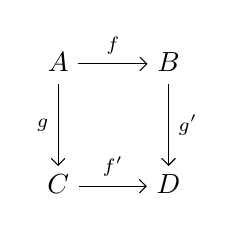
\begin{tikzpicture}[>=angle 90]
\matrix(a)[matrix of math nodes,
row sep=3em, column sep=2.5em,
text height=1.5ex, text depth=0.25ex]
{
A & B \\
C & D \\};
\path[->,font=\scriptsize]
(a-1-1) edge node[above]{$f$} (a-1-2)
(a-1-1) edge node[left]{$g$} (a-2-1)
(a-2-1) edge node[above]{$f'$} (a-2-2)
(a-1-2) edge node[right]{$g'$} (a-2-2);
\end{tikzpicture}
\caption{Pullback}
\end{figure}


\end{document}
